\documentclass{problemset}
\usepackage{amsmath}

\usepackage{lipsum}
%\usepackage{showframe}
\usepackage{layout}


\usepackage[charter,cal=cmcal]{mathdesign} %different font
\usepackage{microtype}
\usepackage{amsmath}
%\usepackage{amsfonts}
%\usepackage{amssymb}
\usepackage{graphicx}
\usepackage[inline]{enumitem}
\usepackage{xparse}
\usepackage{ifthen}
\usepackage{graphicx}
\usepackage{caption}
\usepackage{subcaption}
\usepackage{color}
\usepackage{tikz}
\usepackage{fancyhdr}
\usepackage{calc}
\usepackage[hidelinks]{hyperref}

\usepackage{pgfplots}
\pgfplotsset{compat=newest}
%%%
% Useful Linear Algebra macros
%%%
\newcommand{\ul}{$\underline{\phantom{xxx}}$}
\newcommand{\ull}{\underline{\phantom{xxx}}}
\newcommand{\xh}{{\hat {\mathbf x}}}
\newcommand{\yh}{{\hat {\mathbf y}}}
\newcommand{\zh}{{\hat {\mathbf z}}}
\newcommand{\R}{\mathbb{R}}
\newcommand{\Z}{\mathbb{Z}}
\newcommand{\N}{\mathbb{N}}
\newcommand{\proj}{\mathrm{proj}}
\newcommand{\Proj}{\mathrm{proj}}
\newcommand{\Perp}{\mathrm{perp}}
\renewcommand{\span}{\mathrm{span}\,}
\newcommand{\Span}{\mathrm{span}\,}
\newcommand{\Img}{\mathrm{img}\,}
\newcommand{\Null}{\mathrm{null}\,}
\newcommand{\Range}{\mathrm{range}\,}
\newcommand{\rref}{\mathrm{rref}}
\newcommand{\rank}{\mathrm{rank}}
\newcommand{\Rank}{\mathrm{rank}}
\newcommand{\nnul}{\mathrm{nullity}}
\newcommand{\mat}[1]{\begin{bmatrix}#1\end{bmatrix}}
\newcommand{\chr}{\mathrm{char}}
\renewcommand{\d}{\mathrm{d}}

%\tcbuselibrary{skins}
%\usetikzlibrary{shadings}


%%%
% Set up the margins to use a fairly large area of the page
%%%
\textwidth=6in
\topmargin=-1in
\textheight=10in
\parskip=.07in
\parindent=0in

\begin{document}
\pagestyle{empty}

\begin{center}
{\huge\bf Inquiry Based Vector Calculus}\\

\vspace{.7in}
{
\it \copyright\,Jason Siefken, 2015 \\
Creative Commons By-Attribution Share-Alike\, \makebox(30,5){\includegraphics[height=1.2em]{by-sa.pdf}}
}
\end{center}

\section*{About the Document}

	This document was originally designed in the fall of 2015 to guide students
	through an eleven week Vector Calculus course (Math 281-1) at
	Northwestern University.  

	A typical class day using the problem-sets:
	\begin{enumerate}
		\item {\bf Introduction by instructor.} This may involve giving a definition,
			a broader context for the day's topics, or answering questions.
		\item {\bf Students work on problems.} Students work individually or in pairs
			on the prescribed problem.  During this time the instructor moves around
			the room addressing questions that students may have and giving one-on-one
			coaching.
		\item {\bf Instructor intervention.} If most students have successfully solved the 
			problem, the instructor regroups the class by providing a concise 
			explanation so that everyone is ready to move to the next concept.  This
			is also time for the instructor to ensure that everyone has understood the
			main point of the exercise (since it is sometimes easy to do some computation
			while being oblivious to the larger context).

			If students are having trouble, the instructor can give hints to the group,
			and additional guidance to ensure the students don't get frustrated
			to the point of giving up.
		\item {\bf Repeat step 2.}
	\end{enumerate}

	Using this format, students are working (and happily so) most of the class.
	Further, they are especially primed to hear the insights of the instructor, 
	having already invested substantially into each problem.

	This problem-set is geared towards concepts instead of computation, though some problems
	focus on simple computation.

	{\bf License}  This document is licensed under the Creative Commons
	By-Attribution Share-Alike License.  That means, you are free to use,
	copy, and modify this document provided that you provide attribution
	to the previous copyright holders and you release your derivative work 
	under the same license.  Full text of the license is at \url{http://creativecommons.org/licenses/by-sa/4.0/}

	If you modify this document, you may add your name to the copyright list.  Also,
	if you think your contributions would be helpful to others, consider making a pull
	requestion, or opening an \emph{issue} at 
	\url{https://github.com/siefkenj/IBLVectorCalculus}


\newpage

\setcounter{page}{1}
\pagestyle{fancy}
\rfoot{\footnotesize\it \copyright\,Jason Siefken, 2015--2016 \ \makebox(30,5){\includegraphics[height=1.2em]{by-sa.pdf}}}
\renewcommand{\headrulewidth}{0pt}

\section*{Vectors}

	\question
	\begin{tikzpicture}[>=latex,scale=4]
		\draw[style=help lines] (0,0) (2,2);

		\draw[->,thick,black] (0,0) -- (135:1) node [left] {$\mathbf a$};
		\draw[->,thick,black] (0,0) -- (0,1) node [left] {$\mathbf b$};
		\draw[->,thick,black] (0,0) -- (45:1) node [above] {$\mathbf c$};
		\draw[->,thick,black] (0,0) -- (1,0) node [above] {$\mathbf d$};
		\draw (0,0) node [below] {$\mathbf o$};
		
		\draw[thick,blue,fill] (1,2) circle [radius=.02] node [below right,black] {$p$};
		\draw[thick,blue] (2,1) circle [radius=.02] node [below right,black] {$q$};

	\end{tikzpicture}

	Notice that all arrows in this diagram are the same length.
	We will call this length a \emph{unit}.
	\begin{parts}
		\item Give directions from $\bf o$ to $p$ of
		the form ``Walk \ul units in the direction of arrow \ul, then 
		walk \ul units in the direction of arrow \ul.''

		\item Can you give directions with the two arrows you haven't
		used?  Give such directions, or explain why it cannot be done.

		\item Give directions from $\bf o$ to $q$.

		\item Can you give directions from $\bf o$ to $q$ using $\bf c$ and $\bf a$?
		Give such directions, or explain why it cannot be done.

	\end{parts}

	\question
	\begin{minipage}{.35\textwidth}
	\begin{tikzpicture}[>=latex,scale=4]
		\draw[style=help lines] (0,0) (1,2);

		\draw[->,thick,black] (0,0) -- (0,1) node [left] {$\yh$};
		\draw[->,thick,black] (0,0) -- (63.4:1) node [left] {$\mathbf c$};
		\draw[->,thick,black] (0,0) -- (1,0) node [above] {$\xh$};
		\draw (0,0) node [below] {$\mathbf o$};
		
		\draw[thick,blue,fill] (1,2) circle [radius=.02] node [below right,black] {$p$};

	\end{tikzpicture}
	\end{minipage}
	\begin{minipage}{.65\textwidth}
	We are going to start using a more mathematical notation
	for giving directions.  Our directions will now look like
	\[
		p = \ull\, \xh + \ull\, \yh
	\]
	which is read as ``To get to $p$ (=) go \ul units in the direction $\xh$ then (+) go \ul units in 
	the direction $\yh$.''

	\begin{parts}
		\item What is the difference between $p = \ull\, \xh + \ull\, \yh$ and $p = \ull\, \yh + \ull\, \xh$?
		Can they both give valid directions?
		\item
		\begin{enumerate}
			\item Give directions to $p$ using the new notation. 
			\item Give directions to $p$ using $\bf c$.  (Notice that
				$\bf c$ points directly at $p$.)
			\item What is the distance from $\bf o$ to $p$ in units?
		\end{enumerate}
		\item
		\begin{enumerate}
			\item $r=1\bf c$.  Give directions from $\bf o$ to $r$ using $\xh$ and $\yh$.
			\item What is the distance from $\bf o$ to $r$?
		\end{enumerate}
		\item
		\begin{enumerate}
			\item $q=-2\xh+3\yh$; find the exact distance from $\bf o$ to $q$.
			\item $s=2\xh+\bf c$; find the exact distance from $\bf o$ to $s$.
		\end{enumerate}
	\end{parts}
	\end{minipage}


	The vectors $\xh$ and $\yh$ are called the \emph{standard
	basis vectors} for $\R^2$ (the plane).  

\section*{Column Vector Notation}
	We previously wrote $q=-2\xh+3\yh$.  In column vector notation we write
	\[
		q=\begin{bmatrix}-2\\3\end{bmatrix}
	\]
	We may call $q$ either a \emph{vector} or a \emph{point}.  If we call $q$ a vector,
	we are emphasizing that $q$ gives direction of some sort.  If we call $q$ a point,
	we emphasize that $q$ is some absolute location in space. (What's the philosophical
	difference between a location in space and directions from the origin to said location?)

	\question 
	$r=1\bf c$ and $s=2\xh+\bf c$ where $\bf c$ is the vector from before.
	\begin{parts}
		\item Write $r$ and $s$ in column vector form.
	\end{parts}

\section*{Sets and Set Notation}

	\begin{definition}[Set]
		A \emph{set} is a (possibly infinite) collection of items
		and is notated with curly braces (for example, $\{1,2,3\}$ is
		the set containing the numbers 1, 2, and 3).  We call the items in
		a set \emph{elements}.

		If $X$ is a set and $a$ is an element $X$, we may write $a\in X$,
		which is read ``$a$ is an element of $X$.''

		If $X$ is a set, a \emph{subset} $Y$ of $X$ (written $Y\subseteq X$)
		is a set such that every element of $Y$ is an element of $X$.

		We can define a subset using \emph{set-builder notation}.
		That is, if $X$ is a set, we can define the subset 
		\[
			Y= \{a\in X:\text{some rule involving }a\},
		\]
		which is read ``$Y$ is the set of $a$ in $X$ {\bf such that} some rule
		involving $a$ is true.''  If $X$ is intuitive, we may omit it and
		simply write $Y=\{a:\text{some rule involving }a\}$.  You may equivalently
		use ``$|$'' instead of ``$:$'', writing $Y=\{a\,|\,\text{some rule involving }a\}$.
	\end{definition}

	\begin{definition}
		Some common sets are
		\begin{itemize}
			\item[] $\N=\{\text{natural numbers}\} = \{\text{non-negative whole numbers}\}$.
			\item[] $\Z=\{\text{integers}\} = \{\text{whole numbers, including negatives}\}$.
			\item[] $\R=\{\text{real numbers}\}$.
			\item[] $\R^n=\{\text{vectors in $n$-dimensional Euclidean space}\}$.
		\end{itemize}
	\end{definition}


	\question
	\begin{parts}
		\item Which of the following are true?
		\begin{enumerate}
			\item $3\in\{1,2,3\}$.
			\item $1.5\in\{1,2,3\}$.
			\item $4\in\{1,2,3\}$.
			\item ``b''$\in\{x:x\text{ is an English letter}\}$.
			\item ``\`o''$\in\{x:x\text{ is an English letter}\}$.
			\item $\{1,2\}\subseteq \{1,2,3\}$.
			\item For some $a\in\{1,2,3\}$, $a \geq 3$.
			\item For any $a\in\{1,2,3\}$, $a\geq 3$.
			\item $1\subseteq\{1,2,3\}$.
			\item $\{1,2,3\}=\{x\in\R:1\leq x\leq 3\}$.
			\item $\{1,2,3\}=\{x\in\Z:1\leq x\leq 3\}$.
		\end{enumerate}
	\end{parts}

	\question
		Write the following in set-builder notation
	\begin{parts}
			\item The subset $A\subseteq \R$ of real numbers larger than $\sqrt{2}$.
			\item The subset $B\subseteq \R^2$ of vectors whose first coordinate
			is twice the second.
	\end{parts}

	\begin{definition}[Unions \& Intersections]
		Two common set operations are \emph{unions} and \emph{intersections}.  
		Let $X$ and $Y$ be sets.

		\hfill\begin{minipage}{\dimexpr\textwidth-3cm}
		\begin{itemize}
			\item[(union)] $X\cup Y = \{a:a\in X\text{ or }a\in Y\}$.
			\item[(intersection)] $X\cap Y = \{a: a\in X\text{ and }a\in Y\}$.
		\end{itemize}
		\end{minipage}
	\end{definition}

	\question
	Let $X=\{1,2,3\}$ and $Y=\{2,3,4,5\}$ and $Z=\{4,5,6\}$.  Compute
	\begin{parts}
		\item $X\cup Y$
		\item $X\cap Y$
		\item $X\cup Y\cup Z$
		\item $X\cap Y\cap Z$
	\end{parts}

	\question
	Draw the following subsets of $\R^2$.
	\begin{parts}
		\item $V=\left\{\vec x\in\R^2:\vec x=\begin{bmatrix}0\\t\end{bmatrix}\text{ for some }t\in\R\right\}$.
		\item $H=\left\{\vec x\in\R^2:\vec x=\begin{bmatrix}t\\0\end{bmatrix}\text{ for some }t\in\R\right\}$.
		\item $J=\left\{\vec x\in\R^2:\vec x=t\begin{bmatrix}1\\1\end{bmatrix}\text{ for some }t\in\R\right\}$.
		\item $V\cup H$.
		\item $V\cap H$.
		\item Does $V\cup H=\R^2$?
	\end{parts}


\section*{Dot Product}

	\begin{definition}[Dot Product]
	If $\vec a=\begin{bmatrix}a_1\\ a_2\\ \vdots \\ a_n\end{bmatrix}$ and 
	$\vec b=\begin{bmatrix}b_1\\ b_2\\ \vdots \\ b_n\end{bmatrix}$ are two vectors in $n$-dimensional
		space, then the \emph{dot product} of $\vec a$ an $\vec b$ is
	\[
		\vec a\cdot\vec b = a_1b_1+a_2b_2+\cdots+a_nb_n.
	\]
	Equivalently, the dot product is defined by the geometric formula
	\[
		\vec a\cdot \vec b = \|\vec a\|\|\vec b\|\cos \theta
	\]
	where $\theta$ is the angle between $\vec a$ and $\vec b$.
	\end{definition}
	
	\question
		Let $\vec a=\begin{bmatrix}1\\1\end{bmatrix}$, $\vec b=\begin{bmatrix}3\\2\end{bmatrix}$, and $\vec u=\begin{bmatrix}1\\2\\1\end{bmatrix}$.
	\begin{parts}
		\item 
		\begin{enumerate}	
			\item Draw a picture of $\vec a $ and $\vec b$.
			\item Compute $\vec a\cdot \vec b$.
			\item Find $\|\vec a\|$ and $\|\vec b\|$ and use your knowledge of
			the multiple ways to compute the dot product to find $\theta$,
			the angle between $\vec a$ and $\vec b$. Label $\theta$ on your picture.
		\end{enumerate}
		\item Draw the graph of $\cos$ and identify which angles make $\cos$ negative, zero,
		or positive.

		\item Draw a new picture of $\vec a$ and $\vec b$ and on that picture draw
		\begin{enumerate}	
			\item a vector $\vec c$ where $\vec c\cdot \vec a$ is negative.
			\item a vector $\vec d$ where $\vec d\cdot \vec a=0$ and $\vec d\cdot \vec b < 0$.
			\item a vector $\vec e$ where $\vec e\cdot \vec a=0$ and $\vec e\cdot \vec b>0$.
			\item Could you find a vector $\vec f$ where $\vec f\cdot \vec a=0$ and $\vec f\cdot \vec b=0$?
			Explain why or why not.
		\end{enumerate}

		\item Recall the vector $\vec u$ whose coordinates are given at the beginning of this problem.
		\begin{enumerate}
			\item Write down a vector $\vec v$ so that the angle between $\vec u$ and $\vec v$
			is $\pi/2$. (Hint, how does this relate to the dot product?)
			\item Write down another vector $\vec w$ (in a different direction from $\vec v$)
			so that the angle between $\vec w$ and $\vec u$ is $\pi/2$.
			\item Can you write down other vectors different than both $\vec v$ and $\vec w$ that still
			form an angle of $\pi/2$ with $\vec u$?  How many such vectors are there?
		\end{enumerate}
	\end{parts}

	\begin{definition}[Norm]
		The \emph{norm} of a vector $\vec v\in\R^n$, denoted $\|\vec v\|$ is its length
		and is given by the formula
		\[
			\|\vec v\| = \sqrt{\vec v\cdot\vec v}.
		\]
	\end{definition}

	\question
	\begin{parts}
		\item Let $\vec a = \mat{3\\2}$.  Find $\|\vec a\|$ using the Pythagorean theorem
			and using the formula from the definition of the norm.  How do
			these quantities relate?
		\item Let $\vec b = \mat{1\\1\\-2\\2}$, and find $\|\vec b\|$.
		Did you know how to find 4-d lengths before?
	
		\item Suppose $\vec u=\mat{x\\ y}$ for some $x,y\in \R$.
		Could $\vec u\cdot \vec u$ be negative? Compute $\vec u\cdot \vec u$ algebraically
		and use this to justify your answer.
	\end{parts}

	\begin{definition}[Distance]
		The \emph{distance} between two vectors $\vec u$ and $\vec v$ is $\|\vec u-\vec v\|$.
	\end{definition}
	\begin{definition}[Unit Vector]
		A vector $\vec v$ is called a \emph{unit vector} if $\|\vec v\|=1$.
	\end{definition}
	
	\question
	Let $\vec u=\mat{1\\2\\1}$ and $\vec v=\mat{1\\1\\3}$.
	\begin{parts}
		\item Find the distance between $\vec u$ and $\vec v$.
		\item Find a unit vector in the direction of $\vec u$.
		\item Does there exists a \emph{unit vector} $\vec x$ that is distance
			$1$ from $\vec u$?
		\item Suppose $\vec y$ is a unit vector and the distance between $\vec y$ and
			$\vec u$ is $2$.  What is the angle between $\vec y$ and $\vec u$?
	\end{parts}

	\begin{definition}[Orthogonal]
		Two vectors $\vec u$ and $\vec v$ are \emph{orthogonal} to each other
		if $\vec u\cdot \vec v=0$.  The word orthogonal is synonymous with the
		word perpendicular.
	\end{definition}

	\newpage
	\question
	\begin{parts}
		\item Find two vectors orthogonal to $\vec a=\mat{1\\-3}$.  Can you find two such vectors that
			are not parallel?
		\item Find two vectors orthogonal to $\vec b=\mat{1\\-3\\4}$.  Can you find two 
			such vectors that are not parallel?
		\item Suppose $\vec x$ and $\vec y$ are orthogonal to each other and $\|\vec x\|=5$ and $\|\vec y\|=3$.
			What is the distance between $\vec x$ and $\vec y$?
	\end{parts}


\section*{Projections}
	Projections (sometimes called orthogonal projections) are a way to measure how much one vector
	points in the direction of another.

	\begin{definition}[Projection]
	\begin{center}
	\usetikzlibrary{patterns,decorations.pathreplacing}
	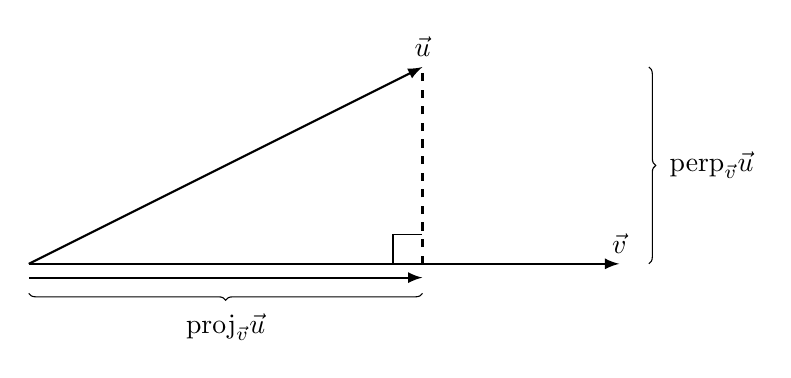
\begin{tikzpicture}[>=latex,scale=2.5]
		\draw[->,thick,black] (0,0) -- (2,1) node [above] {$\vec u$};
		\draw[->,thick,black] (0,0) -- (3,0) node [above] {$\vec v$};
		\draw[->,thick,black,yshift=-.07cm] (0,0) -- (2,0);
		\draw[decoration={brace, mirror}, decorate, yshift=-.15cm] (0,0) -- (2,0) node [midway,below,yshift=-4pt] {$\Proj_{\vec v}\vec u$};
		
		\draw[dashed,thick,black] (2,0) -- (2,1);
		\draw[decoration={brace, mirror}, decorate, xshift=1.15cm] (2,0) -- (2,1) node [midway,right,xshift=4pt] {$\Perp_{\vec v}\vec u$};
		\draw[thin,black] (1.85,0)--(1.85,.15)--(2,.15);

	\end{tikzpicture}
	\end{center}
	\vspace{-.6cm}
	
	The \emph{projection} of $\vec u$ onto $\vec v$ is written $\proj_{\vec v}\vec u$ and is the vector in the direction of $\vec v$
	such that $\vec u-\Proj_{\vec v}\vec u$ is orthogonal to $\vec v$.  The vector $\vec u-\Proj_{\vec v}$ is called the \emph{perpendicular
	component} of $\vec u$ with respect to $\vec v$ and is notated as $\Perp_{\vec v}\vec u$.
	\end{definition}
	
	\question
	\begin{center}
	\usetikzlibrary{patterns,decorations.pathreplacing}
	\begin{tikzpicture}[>=latex,scale=2.5]
		\draw[->,thick,black] (0,0) -- (30:2) node [above] {$\vec a$};
		\draw[->,thick,black] (0,0) -- (3,0) node [above] {$\vec b$};
		\draw[thick,black] (0,0) +(0:.3cm) arc (0:30:.3cm) node[right,yshift=-4pt] {$\theta$};

	\end{tikzpicture}
	\end{center}


	In this picture $\|\vec a\|=4$, $\theta = \pi/6$, and $\vec b=\mat{6\\0}$.
	%%%
	% XXX: This is confusing with multiple b vectors. Should instead emphasise that proj_b(a ) = proj_{-b}(a).
	%%%
	\begin{parts}
		\item   Write $\vec a$ in column vector form.
		\item   Find $\|\Proj_{\vec b}\vec a\|$ and $\|\Perp_{\vec b}\vec a\|$.
		\item Write down 
				$\Proj_{\vec b}\vec a$ and $\Perp_{\vec b}\vec a$ in column vector
				form.
		\item If $\vec c=\mat{-4\\0}$, write down 
				$\Proj_{\vec c}\vec a$ and $\Perp_{\vec c}\vec a$ in column vector
				form.
		\item If $\vec d=\mat{3\\1}$, write down 
				$\Proj_{\vec d}\vec a$ and $\Perp_{\vec d}\vec a$ in column vector
				form.  (You may need to use your knowledge of how dot products and angles
				relate to answer this one.)
		\item Consider $\vec d=\mat{3\\1}$.  Compute $\proj_{\xh}\vec d$ and 
		$\proj_{\yh}\vec d$.  How do these projections relate to the coordinates of $\vec d$? What
		can you say in general about projections onto $\xh$ and $\yh$?
	\end{parts}


\section*{Lines, Planes, Normals, and Equations}

	\question
	\begin{parts}
		\item Draw $\vec u=\begin{bmatrix}2\\3\end{bmatrix}$ and \emph{all}
		vectors perpendicular to it.
		\item If $\vec x=\begin{bmatrix}x\\y\end{bmatrix}$ and $\vec x$ is 
		perpendicular to $\vec u$, what is $\vec x\cdot \vec u$?
		\item Expand the dot product $\vec u\cdot \vec x$ to get an equation
		for a line.  This equation is called the \emph{scalar equation} representing the line.
	\end{parts}

	\begin{definition}[Normal Vector]
		A \emph{normal vector} to a line (or plane or hyperplane) is a non-zero vector that is orthogonal to it.
	\end{definition}

	\begin{parts}[resume]
		\item Rewrite the line $\vec u\cdot \vec x = 0$ in $y=mx+b$ form and verify it matches
		the line you drew above.
	\end{parts}

	\question
	We can also write a line in \emph{parametric form} by introducing a parameter
	that traces out the line as the parameter runs over all real numbers.
	\begin{parts}
		\item Draw the line $L$ with $x,y$ coordinates given by
		\[
			\begin{array}{l}x=t\\y=2t\end{array}
		\]
		as $t$ ranges over $\R$.
		\item Write the line $\vec u \cdot \vec x=0$ (where $\vec u$ is the same as before) in parametric form.
	\end{parts}
	
	\question
	\emph{Vector form} is the same as parametric form but written in vector notation.  For example, the
	line $L$ from earlier could be written as 
	\[
		\begin{bmatrix}x\\y\end{bmatrix}=\begin{bmatrix}t\\2t\end{bmatrix}
	\]
	or
	\[
		\begin{bmatrix}x\\y\end{bmatrix}=t\begin{bmatrix}1\\2\end{bmatrix}.
	\]

	\begin{parts}
		\item Write the line $\vec u\cdot \vec x=0$ in vector form.  That is, find a vector $\vec v$ so
		the line $\vec u\cdot \vec x=0$  can be written as
		\[
			\begin{bmatrix}x\\y\end{bmatrix} = t\vec v
		\]
		as $t$ ranges over $\R$.
		\item What is $\vec v\cdot \vec u$? Why? Will this always happen?
	\end{parts}


	\subsection*{Moving to Planes}
	
	\question
	\begin{parts}
		\item Write down three solutions $\vec a$, $\vec b$, $\vec c\in\R^3$ to
		\begin{equation}\label{eq1}
			2x+y-z=0.
		\end{equation}
		\item Find $\vec n\in\R^3$ so that equation (\ref{eq1}) is equivalent
		to $\vec n\cdot \vec x=0$ where $\vec x=\begin{bmatrix}x\\ y\\ z\end{bmatrix}$.
		\item What do you notice about the angle between solutions to equation (\ref{eq1}) and $\vec n$?
	\end{parts}

	When writing down solutions to equation (\ref{eq1}), you got to choose two coordinates before the remaining
	coordinate became determined.  This means the solutions have two parameters (and consequently form a
	two dimensional space).

	\begin{parts}[resume]
		\item Write down parametric form of a line of solutions to equation (\ref{eq1}).
		\item Write down parametric form of a different line of solutions to equation (\ref{eq1}).
		\item Write down all solutions to equation (\ref{eq1}) in parametric form.  That is, find $a_x,
		a_y,a_z,b_x,b_y,b_z$ so that
		\[
			\begin{array}{l}
				x=a_x t+b_x s\\
				y=a_y t+b_y s\\
				z=a_z t+b_z s
			\end{array}
		\]
		gives all solutions as $t,s$ vary over all of $\R$.
		\item Write all solutions to equation (\ref{eq1}) in vector form.
	\end{parts}

\subsection*{Arbitrary Lines and Planes}
	
	So far, all of our lines and planes have passed through the origin. To 
	produce the equation of an arbitrary line/plane, we first make one of
	same ``slope'' that passes through the origin, then we translate it
	to the appropriate place.

	\question
	We'd like to write the equation of a line $L$ with normal vector
	$\vec n=\begin{bmatrix}4\\-1\end{bmatrix}$ that passes through
	the point $p=\mat{-1\\-1}$

	\begin{parts}
		\item Give a scalar equation of the line $L_2$ which is parallel to $L$
		but passes through the origin.
		\item Draw a picture of $L$ and $L_2$, and find two points that lie on
		$L$.  Call these points $p_1$ and $p_2$.
		\item Verify the vector $\overline {p_1p_2}$ is orthogonal to $\vec n$.
		\item What is $\vec n\cdot p_1$, $\vec n\cdot p_2$, $\vec n\cdot p$?
		Should these values be zero, equal, or different?  Explain (think about
		projections).
		\item How does the equation $\vec n\cdot (\vec x-p)=0$ relate to $L$?
	\end{parts}

	\question
	$W$ is the plane with normal vector $\vec n=\mat{1\\2\\3}$ and that passes through
	the point $p=\mat{1\\1\\2}$.
	\begin{parts}
		\item Write normal form of $W$.
		\item Write vector form of $W$.
	\end{parts}


\section*{Arc Length}

	\question
	The parameterized curve
	\[
		\vec r(t) = \mat{2\cos t\\2\sin t}
	\]
	describes the position of a particle at time $t$.
	\begin{parts}
		\item Describe the path and motion of this particle in words.
		\item Compute the displacement  of the particle between $t=0$
			and $t=\Delta t$ and call the resulting vector $\Delta \vec r$.  
			(Assume $\Delta t$ is small.)
		\item Approximate the length of $\Delta \vec r$.  You may use the fact that
			\[
				\sin x\approx x\qquad\text{and}\qquad \cos x\approx -\tfrac{1}{2}x^2+1
			\]
			when $x\approx 0$.
		\item Use a limit to compute the velocity of the particle at $t=0$. Call this 
			vector $\vec v_0$.
		\item Use a limit to compute the speed at $t=0$.  Call this value $s_0$.
		\item How do $\|\vec v_0\|$ and $s_0$ relate?  Why?
	\end{parts}

	\question
	A particle's path is parameterized by
	\[
		\vec m(t) = (f(t), g(t), h(t))
	\]
	where $t$ represents time.
	\begin{parts}
		\item Derive (with explanation) a formula for the velocity of
			the particle at time $t=t_0$.
		\item Derive (with explanation) a formula for the speed of
			the particle at time $t=t_0$.
	\end{parts}
	
	\question
	Recall the particle whose path is given by
	$
		\vec r(t) = \mat{2\cos t\\2\sin t}
	$
	where $t$ represents time.
	\begin{parts}
		\item Use the fact that
			\[
				\text{distance traveled}=\int\text{\it speed}\ \mathrm{d}\text{\it time}
			\]
		to produce a formula for how far the particle has traveled from $t=0$ to $t=t_0$.
		\item Use geometry to do the same thing.
		\item Derive an expression (with explanation) for the arc length of $\vec m(t) = (f(t), g(t), h(t))$
			from $t=0$ to $t=t_0$.
	\end{parts}

\subsection*{Arc Length Parameterization}
	
	An \emph{arc length parameterization} of a curve $C$ is a function $\vec s:\R\to\R^n$ whose
	image is $C$ with the added property that the arc length of $\vec s(t)$ from $t=0$ to $t=t_0$
	is $t_0$ for all valid choices of $t_0$.  I.e., the distance traveled by the parameter along
	$\R$ is the same as the distance traveled by the point $\vec s(t)$ in $\R^n$.

	\question
	\begin{parts}
		\item Produce an arc length parameterization of the curve parameterized by
			$
				\vec r(t) =\mat{2\cos t\\ 2\sin t}.
			$
		\item Produce an arc length parameterization of the curve parameterized by
			$
				\vec q(t) =\mat{t\\ t^{3/2}}.
			$
	\end{parts}

	
	An arc length parameterization of a curve can also be thought of
	as a parameterization where a particle always moves at unit speed 
	(if you interpret a parameterized curve as describing the motion of a
	particle).

	By reparameterizing, we can describe the motion of a particle along
	a path at any speed.

	\question
	A particle moves along a path $C$, which is a circle in $\R^2$ of radius $3$, centered at the origin, and oriented counter-clockwise.
	\begin{parts}
		\item Parameterize $C$ so that the speed is $2.5$.
		\item Parameterize $C$ so that the speed of the particle starts and ends at $0$.
		\item Parameterize $C$ so that the speed of the particle starts at $0$ and ends at $4$.
		\item Parameterize $C$ so that the speed of the particle is $0$ at six points along the curve.
	\end{parts}

	\question
	A particle's motion is described by the function $\vec h(t) = \mat{f(t)\\ g(t)}$,  which is a 
	parameterization of the curve $H$.  The arc length of $H$ from $t=0$ to
	$t=t_0$ using this parameterization is given by the function $s(t_0) = t_0^2$.
	\begin{parts}
		\item Write an expression for the speed of the particle at time $t$.
		\item Give a formula for the arc length parameterization of $H$.
	\end{parts}




\section*{Tangents, Normals, and Acceleration}
	
	\begin{definition}[Velocity \& Acceleration]
	Suppose $\vec r(t)$ describes the motion of a particle.  The \emph{velocity}
	of the particle is defined as
	\[
		\vec v(t) = \lim_{h\to 0} \frac{\vec r(t+h)-\vec r(t)}{h}.
	\]
	The \emph{acceleration}
	of the particle is defined as
	\[
		\vec a(t) = \lim_{h\to 0} \frac{\vec v(t+h)-\vec v(t)}{h}.
	\]
	\end{definition}
	Both $\vec v$ and $\vec a$ are vector-valued derivatives.

	\question
	Let $\vec r(t) = \mat{t+2\\ \sin t\\ t^3}$ represent the position of a particle at time $t$.
	\begin{parts}
		\item Find the velocity of the particle at time $t$.
		\item Find the acceleration of the particle at time $t$.
	\end{parts}

	\question
	Let $\vec r_\ell(t) = \mat{\frac{t^2}{2}\\\frac{t^2}{2}}$ and $\vec r_c(t) = \mat{\cos t\\ \sin t}$ represent the position
	of the particles $r_\ell$ and $r_c$ at time $t$.
	\begin{parts}
		\item Describe the paths of each of these particles.  What should their accelerations be?  Why?
		\item Compute the accelerations of $r_\ell$ and $r_c$ at time $t$.
		\item Compute the tangent vectors for the functions $\vec r_\ell$ and $\vec r_c$ at time $t$.
			How does the direction of the tangent vectors and the direction of the acceleration vectors
			compare?
	\end{parts}

	If $\vec r(t)$ describes the position of a particle at time $t$ and $\vec a(t)$ its acceleration, $\vec a(t)$
	can be decomposed into a \emph{tangential} component, $\vec a_T(t)$, and a \emph{normal} component $\vec a_N(t)$
	so that
	\[
		\vec a(t) = \vec a_T(t) +\vec a_N(t).
	\]

	\question
	Let $\vec r_{p}(t) = \mat{t\\ t^2}$  represent the position
	of the particle $\vec r_{p}$ at time $t$.
	\begin{parts}
		\item Compute the tangential and normal components of the acceleration of $\vec r_{p}$.
		\item By changing the speed of $\vec r_{p}$ (but not its path), is it possible to make 
			the tangential component of its acceleration zero?
		\item By changing the speed of $\vec r_{p}$ (but not its path), is it possible to make 
			the normal component of its acceleration zero?
	\end{parts}

	We're going to develop some tools to mathematically verify our intuition about the acceleration
	vector.

	\question
	\begin{parts}
		\item Suppose $\vec p(t)$ and $\vec q(t)$ are both vector-valued functions.  Expand $\vec p(t)\cdot\vec q(t)$
		using components. Now, come up with an expression for $\Big(\vec p(t)\cdot\vec q(t)\Big)'$.  Look at your
		result and rewrite it as an expression involving dot products.
		You've just discovered a product rule for the dot product!
		\item Using similar methods to the computation of $\Big(\vec p(t)\cdot\vec q(t)\Big)'$, find an expression
			for $\|\vec p(t)\|'$.
		\item If a particle whose path is given by $\vec r(t)$ is moving at unit speed, then $\|\vec v(t)\| = 1$.
			Take derivatives of both sides of this expression to show that $\vec v(t)\cdot \vec a(t) = 0$.
	\end{parts}



\section*{Visualizing Surfaces}
	As we've already seen, being able to picture multi-dimensional objects is 
	invaluable when intuiting solutions and when coming up with mathematical
	justifications for intuition.  There are two main ways we visualize
	2D surfaces: perspective drawings and level-curves.


	\question
		Consider the surface defined by $z=f(x,y)$ where $f(x,y)=x^2+y^2$.
	\begin{parts}
		\item On a single $xy$-plane, draw the set of points satisfying the equations $0=f(x,y)$, $1=f(x,y)$,
			$2=f(x,y)$, $3=f(x,y)$, and $4=f(x,y)$.  What is the set of points satisfying $-1=f(x,y)$?
	\end{parts}
	The curves you just drew are called \emph{level curves}.
	\begin{parts}[resume]
		\item Plot in 3D the function $z=f(x,y)$ for $z=0,1,2,3,4$.  Are you able to see what this surface looks like?
		\item We can plot more and more contours of this surface until we have a good idea of what it looks like.
			Add the set of points $z=f(0,y)$ and $z=f(x,0)$ to your plot.
	\end{parts}


	\question
	Level curves are contours produced by fixing $z$ and graphing the result.  Other useful contours
	come about by fixing $x$ or $y$.  Use any contour-based method to plot the following surfaces.
	\begin{parts}
		\item $z=x^2-y^2$
		\item $z^2=4x^2+y^2$
		\item $z^2=9-(4x^2+y^2)$
		\item $z=(\sin x)(\sin y)$
	\end{parts}

\newpage
\section*{Directional Derivatives}

	\question
	It is winter in Chicago.  Imagine a bug crawling along the floor of
	a room that is $7\times 7$ meters.  Figure \ref{heatcontour1} shows the contour plot of the heat
	of the floor in Fahrenheit.\footnote{The bug questions are due to Mairead Greene, Amy Ksir, and Christine von Renesse.}
	\begin{figure}[h!]
		\begin{center}
			\includegraphics[width=3.5in]{heat_contour1.pdf}
		\end{center}
		\vspace{-.5cm}
		\caption{Heat contours for a room.}
		\label{heatcontour1}
	\end{figure}
	\begin{parts}
		\item Where is the door to the outside?  Where is the window?  Where is the heater? Why?
			What might be in the lower right corner of the room?
		\item The bug would like to crawl from the window to the right wall along a path that minimizes
			the change in temperature.  Draw two such paths.
		\item The bug makes a circuit around the entire room by walking along the walls clockwise.
			Draw a graph of distance verses temperature for this part of the bug's journey.  How
			do the starting values and ending values of your graph compare?  Is the accuracy of your
			graph limited?
	\end{parts}
	
	\question Figure \ref{heatcontour2} shows the path the bug decided to follow.
	\begin{figure}[h!]
		\begin{center}
			\includegraphics[width=3.5in]{heat_contour2.pdf}
		\end{center}
		\vspace{-.5cm}
		\caption{Heat contours for a room.}
		\label{heatcontour2}
	\end{figure}
	\begin{parts}
		\item Find the average change in temperature from $P$ to $Q$ for the bugs journey.
		\item Estimate the instantaneous rate of change of temperature at the point $P$.
		\item Suppose $T(x,y)$ gives the temperature of the room at the coordinates $(x,y)$.
			Write a limit expression to compute the exact rate of change of temperature
			at the beginning of the bug's journey. Does the rate of change depend on time?
		\item Write a limit expression to compute the rate of change of temperature
			\emph{with respect to distance} at the start of the bug's journey.
		\item If the bug had decided to travel in a different direction, would the rate of change
			of temperature be the same?  Explain.
	\end{parts}
	
	\newpage
	\question
	Let $f(x,y) = 2(x-3)^2+y$
	\begin{parts}
		\item Calculate the rate of change of $f$ at the origin 
			in the directions $\xh$, $\yh$, $\vec a=(\tfrac{\sqrt{2}}{2},\tfrac{\sqrt{2}}{2})$.
		\item Calculate the rate of change of $f$ at $p=(1,-1)$
			in the directions $\xh$, $\yh$, $\vec a=(\tfrac{\sqrt{2}}{2},\tfrac{\sqrt{2}}{2})$.
	\end{parts}





\subsection*{A New Perspective on Derivatives}

	In single-variable calculus, we deal with functions $g:\R\to\R$.  The derivative of this function
	at a point $a$ is the rate of change of $g$ at the point $a$.

	\question
	Let $g(x)=x^2$.
	\begin{parts}
		\item What is the rate of change of $g$ at the points $x=0,1,$ and $2$?  How about at $x=x_0$?
		\item Use your knowledge of the rate of change of $g$ to \emph{approximate} $g(x)$ where
			$x=0+\varepsilon, 1+\varepsilon,$ and $2-\varepsilon$ where $\varepsilon>0$ is a tiny number.
		\item Write down three functions: $G_0$, $G_1$, and $G_2$ so that if $\varepsilon$ is tiny, $g(a+\varepsilon)\approx
			g(a) + G_a(\varepsilon)$.  
	\end{parts}

	\question
	Recall $f(x,y)=2(x-3)^2+y$ from before.
	\begin{parts}
		\item Write down a function $F_{(0,0)}:\R^2\to\R$ such that if $\vec u$ is a vector
			and $\|\vec u\|$ is tiny, 
			\[
				f(\vec 0+\vec u)\approx f(\vec 0) + F_{(0,0)}(\vec u).
			\]
			Notice, $F_{(0,0)}$ is somehow representative of the rate of change of $f$ at $(0,0)$.
			It may help to compute $F_{(0,0)}$ for several example directions before coming up
			with a formula.
		\item Write down a function $F_{(1,-1)}$ so that if $\vec u$ is a vector and $\|\vec u\|$ is
			tiny, $f\Big((1,-1)+\vec u\Big)\approx f(1,-1)+F_{(1,-1)}(\vec u)$.
		\item Can a single number represent the rate of change of $f$ at the point $(0,0)$?  Why or why not?
			If a number cannot, can you think of another object that can?
	\end{parts}

\newpage

	\begin{definition}[Directional Derivative]
		The \emph{directional derivative} of a function $f:\R^n\to\R^m$ at the
		point $\vec a$ in the direction $\vec u$ is
		\[
			D_{\vec a}f(\vec u) = \lim_{h\to 0} \frac{f(\vec a+h\vec u)-f(\vec a)}{h}.
		\]
		I.e., it is the rate of change of $f$ at $\vec a$ heading in the direction of $\vec u$
		with speed $\|\vec u\|$.
	\end{definition}

	\question
	Let $f(x,y) = (x+1)^2+2y$.
	\begin{parts}
		\item Give a parameterization of all two dimensional unit vectors.
		\item Use the definition of the directional derivative to compute
			the directional derivative of $f$ at the point $(0,0)$ in the
			direction of each of your parameterized unit vectors.
		\item Find the direction of the maximal directional derivative.  You
			may find the identity $\sin t+\cos t = \sqrt{2}\sin(t+\tfrac{\pi}{4})$
			helpful.
	\end{parts}

	\begin{definition}[Gradient]
		The \emph{gradient} of a function $f:\R^n\to \R$ is
		\[
			\nabla f  = \left(
				\frac{\partial f}{\partial x_1}, 
				\frac{\partial f}{\partial x_2}, \ldots,
				\frac{\partial f}{\partial x_n}
			\right)
		\]
		where $x_1,\ldots, x_n$ are the parameters of $f$.
	\end{definition}
	
	\question
	Let $f(x,y) = (x+1)^2+2y$ as before.
	\begin{parts}
		\item Compute $\nabla f(0,0)$ (the gradient of $f$ at the point $(0,0)$).
		\item Compute $\nabla f(0,0)\cdot \vec u$ for each of your parameterized unit vectors $\vec u$.
			What do you notice?
		\item Make a conjecture about how the gradient of a function can be used to compute directional derivatives.
	\end{parts}

	\question
	Sticking with $f(x,y) = (x+1)^2+2y$, consider the surface $S=\{\big(x,y,f(x,y)\big):x,y\in\R^2\}$.
	\begin{parts}
		\item Describe $S$.  If $a\in S$, what should \emph{the tangent plane to $S$ at $a$} mean?
		\item Compute the tangent plane, $\mathcal P$, to $S$ at the point $\big(0,0,f(0,0)\big)$ in vector form.
		\item Find standard/normal form of the tangent plane and solve for $z$.  That is,
			find an equation for the tangent plane in the form $z=ax+by+c$.  Do the values $a$, $b$, and
			$c$ look familiar?
		\item Consider the function $g=f-\mathcal P$.  That is, $g(x,y)=f(x,y)-z(x,y)$ where $z(x,y)$ is the
			equation of the tangent plane.  What should the directional derivative of $g$ at $(0,0)$ be?
			Does it depend on direction?
	\end{parts}

	So far, the gradient has been appearing in directional derivatives and tangent planes.
	One might even argue that the gradient \emph{is} the derivative.  Unfortunately, the gradient
	of a function existing is not sufficient for a function to be differentiable.

	\begin{definition}[Differentiable]
		The function $f:\R^n\to \R$ is \emph{differentiable} at $\vec a=(a_1,\ldots,a_n)$ if there exists
		a tangent plane at $\vec a$.  That is, there exists some function $p(x_1,\ldots, x_n)
		= c+\sum \alpha_i (x_i-a_i) = c+\vec \alpha \cdot(\vec x-\vec a)$ so that
		\[
			\lim_{\|\vec u\|\to0} \frac{f(\vec a + \vec u)-p(\vec a + \vec u)}{\|\vec u\|} = 0.
		\]
	\end{definition}

	There's just one trouble with this definition.  How do we take a limit as $\|\vec u\|\to 0$?

\newpage
\subsection*{Multidimensional Limits}

	\begin{definition}[Limit]
		If $f:\R^n\to \R$, then the \emph{limit of $f$ at $\vec a$} exists and is equal to $L$, written
		$\displaystyle \lim_{\vec x\to\vec a} f(\vec x) = L$, if
		for all $\varepsilon > 0$ there exists a $\delta > 0$ such that
		\[
			0<\|\vec x-\vec a\| <\delta \qquad \text{implies}\qquad |f(\vec x) - L| < \varepsilon.
		\]
		If no such $L$ exists, we say the limit does not exist.
	\end{definition}
	When first considered, the definition of limit can be confusing, so let's play with some functions
	that we're familiar with.

	\question
	Let $f(x) = 3x$.
	\begin{parts}
		\item  Draw the graph of $f$ and use your intuition to guess $\lim_{x\to 0} f(x)$.  Call your
			guess $L$.
		\item If $\varepsilon = 1/2$, can you find a $\delta$ so that if $|x-0|<\delta$ we can be assured
			$|f(x)-L|<\varepsilon$?
		\item If $\varepsilon = 1/4$, can you find a $\delta$ so that if $|x-0|<\delta$ we can be assured
			$|f(x)-L|<\varepsilon$?
		\item Come up with a rule for how to choose an appropriate $\delta$ for any $\varepsilon$.
	\end{parts}

	\question
	Let $g(x) = \frac{x}{|x|}$, and let $L$ be a guess for $\lim_{x\to 0} \frac{x}{|x|}$.
	\begin{parts}
		\item Suppose we guess $L=1$.  Picking $\varepsilon = 3/2$, can you find an appropriate
			$\delta$?  What if $L=-1$?  For $\varepsilon=3/2$, can you find an appropriate $\delta$?
			What if $L=0$?  What values can we rule out as possibilities for $L$?
		\item Suppose we guess $L=0$.  Picking $\varepsilon=3/2$, can you find an appropriate $\delta$?
			Is $0$ the limit?  Explain.
		\item Find an $\varepsilon$ that shows that $g$ has no limit at $0$.
	\end{parts}

	\question
	Let $h(x,y) = \frac{xy^2}{x^2+y^2}$.
	\begin{parts}
		\item Give a parameterization of all vectors in $\R^2$ with length $r$.
		\item If $\vec u\in \R^2$ satisfies $\|\vec u\|=r$, can you give upper
			and lower bounds on $h(\vec u)$?
		\item Explain why the limit $\displaystyle \lim_{\|\vec u\|\to 0} h(\vec u)$
			does or doesn't exist.
	\end{parts}
	\question
	Let $h(x,y) = \frac{xy}{x^2+y^2}$.
	\begin{parts}
		\item Give a parameterization of all vectors in $\R^2$ with length $r$.
		\item If $\vec u\in \R^2$ satisfies $\|\vec u\|=r$, can you give upper
			and lower bounds on $h(\vec u)$?
		\item Explain why the limit $\displaystyle \lim_{\|\vec u\|\to 0} h(\vec u)$
			does or doesn't exist.
	\end{parts}


\newpage
\subsection*{Lagrange Multipliers}

	\question
	We know that $\nabla f(\vec a)\cdot \vec u$ gives the directional derivative
	of $f$ at the point $\vec a$ in the direction $\vec u$.  Suppose
	$\nabla f(\vec a) = (1,3)$.
	\begin{parts}
		\item What is the direction of the biggest rate of change of $f$ at $\vec a$? Why?
		\item In what direction is the least change in $f$ at $\vec a$?
	\end{parts}

	\question
	Suppose $C$ is a level curve of $f$.  For $\vec a\in C$, suppose $\vec T_a$ is a tangent vector to
	$C$ at $\vec a$.
	\begin{parts}
		\item What is the rate of change of the function $f$ at $\vec a$ in the direction $\vec T_a$?
		\item What is $\nabla f(\vec a)\cdot \vec T_a$?
		\item If $f(x,y)=x^3+y^2$, find a tangent vector to the curve $C=\{(x,y):f(x,y)=2\}$ at $(1,1)$.
	\end{parts}

	\question
	Consider a function $f:\R^2\to \R$ and a curve $C$ (not a level curve).  Let $\vec r(t)$
	be a parameterization of $C$.  We are interested in the minimum and maximum values for 
	$f\circ \vec r$ (i.e., the min/max values of $f$ on the curve $C$).
	\begin{parts}
		\item What will $(f\circ \vec r)'$ be at a local maximum or minimum?
		\item Explain how to interpret the quantity $(f\circ \vec r)'(t)$
			as a directional derivative.
		\item Use your knowledge of how the gradient allows you to compute directional derivatives
			to come up with a ``chain rule'' for the expression $(f\circ \vec r)'(t)$.
		\item Suppose $f(x,y) = 2x+y$ and $C$ is a circle of radius 1 centered at $\vec 0$.
			Parameterize $C$ and attempt to find the maximum value that $f$ takes on the curve $C$.
			Are these computations easy?
	\end{parts}

	\question
	Let $f(x,y)=2x+y$ and let $C$ be a circle of radius 1 centered at $\vec 0$.
	\begin{parts}
		\item Find a function $g:\R^2\to \R$ so that $C$ is a level curve of $g$.
			Can you pick $g$ so that $C=\{(x,y): g(x,y)=0\}$?
		\item What is the relationship between a tangent vector to $C$ at $\vec a$ and
			$\nabla g(\vec a)$?
		\item Suppose that on the curve $C$, $f$ attains 
			a maximum at $\vec a\in C$. What then is the relationship between 
			$\nabla f(\vec a)$ and $\nabla g(\vec a)$?  Can you describe this relationship
			with a formula?
		\item Use your formula from the previous part along with the constraint $g(x,y)=0$
			to find the maximum value the function $f$ attains on the curve $C$.  Congratulations,
			you've just discovered \emph{Lagrange Multipliers}!

	\end{parts}

	\question
	We will use Lagrange Multipliers to find the dimensions of the largest box (the one with the most volume)
	given that the surface area is $32$.
	\begin{parts}
		\item Write down the function we wish to optimize, call it $f$, and rephrase our constraint
			on surface area so that we may interpret it as the level curve of some function $g$.
		\item Write down a relationship between $\nabla f$ and $\nabla g$ at the maximum.
		\item Write down all equations obtained thus far, and attempt to solve for the dimensions of the box.
			Do we need to solve for every variable?
	\end{parts}
\newpage

\section*{Iterated Integrals}
	Integrals add things up, and iterated integrals are no different; it's just that instead of adding things
	up in one dimension, we add things up in multiple dimensions.

	\question
	To get our bearings, let's revisit integrating with respect of $\mathrm{d}x$ and $\mathrm{d}y$
	when finding area.  Let $T$ be the triangle with vertices $(0,0)$, $(4,0)$, and $(4,3)$.
	\begin{parts}
		\item Draw a picture representing how a Riemann sum could be used to compute the area of $T$.
		\item Draw a picture representing a different way to compute the area of $T$ using a Riemann sum.
		\item Compute the area of $T$ using an integral with respect to $x$; now using an integral with 
			respect to $y$; now using the formula $\frac{1}{2}base\times height$.
	\end{parts}

	\question
	Let $T$ be the triangle with vertices $(0,0)$, $(4,0)$, and $(4,3)$, and imagine that $T$
	outlines a triangular strip of foil.  The density of this foil at any given point (in the 
	first quadrant) is
	$\rho(x,y) = x^2+y$.
	\begin{parts}
		\item Using the fact that for this foil, $mass=density\times area$, write down two different
			integrals that would compute the total mass of $T$, and draw their corresponding
			Riemann-sum pictures.
		\item Evaluate your two integrals.  Is one easier to evaluate than the other?
		\item Can $(x^2+y)\mathrm{d}x\mathrm{d}y$ be interpreted on its own?
	\end{parts}

	\question
	Let the region $R\subset \R^2$ be the area between the parabola $x=y^2$ and the line $x=1$.  Let 
	$f(x,y)=3x+y^2$.
	\begin{parts}
		\item Write down two different iterated integrals to compute $\displaystyle \iint_R f(x,y)\d x\d y$.
		\item Is one of your integrals easier to evaluate than the other?
		\item Describe and draw a region $A$ so that 
			$\displaystyle\iint_A f(x,y)\d x\d y = \int_{x=0}^{x=1}\int_{y=-\sqrt{1-x^2}}^{y=\sqrt{1-x^2}} f(x,y)\d y\d x$.
	\end{parts}

\subsection*{The Volume Form}
	We've been using integrals to find the area or volume (or hypervolume) under a curve.
	Abstractly, this process has been the same every time: chop the region into little pieces, and
	add up each piece's contribution with an integral to find the total.  We're continuing the same
	process, but we're going to start chopping regions up into (sometimes) non-rectangular chunks.

	\question
	\begin{parts}
		\item Draw the lines $x=x_0$, $x=x_0+\Delta x$, $y=y_0$ and $y=y_0+\Delta y$ where
			$\Delta x$ and $\Delta y$ are assume to be small.  Write down a formula for the area enclosed by
			those lines.  Does your formula depend on $x_0$ and $y_0$?
		\item Draw the curves, specified in polar coordinates by $r=r_0$, $r=r_0+\Delta r$, $\theta = \theta_0$,
			and $\theta = \theta_0+\Delta\theta$ where $\Delta r$ and $\Delta \theta$ are assumed to
			be small.  Write down a formula for the area enclosed by those curves.  Does your
			formula depend on $r_0$ and $\theta_0$?
		\item Using the idea that a limit as $\Delta ?\to 0$ of a Riemann sum results in an integral, 
			write down a double-integral expression for the area of a semicircle of radius $1$
			in both rectangular and polar coordinates.
		\item Let $V(r_0,\theta_0) = r_0\Delta r\Delta\theta$, and let $\Delta V(r_0,\theta_0)$ be the exact
			area of the annular (ring-shaped) section you found earlier.  What is $\displaystyle \lim_{\Delta r, \Delta\theta\to 0}
			\frac{\Delta V(r_0,\theta_0)}{V(r_0,\theta_0)}$?  Do we need the $(\Delta r)^2\Delta \theta$ term
			at infinitesimal scales?
	\end{parts}

	\begin{definition}[Volume Form]
		Suppose $\mathcal F$ is a coordinate system for $\R^2$ with a relationship
		to rectangular coordinates given by 
		$x=f_1(a,b)$ and $y=f_2(a,b)$.  The \emph{pre-volume form} associated with $\mathcal F$
		at the point $(a,b)$ is written $\Delta V(a,b)$ and is the area between the curves
		$a=a_0$, $a=a_0+\Delta a$, $b=b_0$, and $b=b_0+\Delta b$.

		The \emph{volume form} associated with $\mathcal F$ at $(a,b)$ is the infinitesimal 
		$\d V(a,b)=V(a,b)\d a\d b$ where $V$ is the unique function satisfying
		\[
			\lim_{\Delta a,\Delta b\to 0} \frac{\Delta V(a,b)}{V(a,b)\Delta a\Delta b} = 1
		\]
		and can obtained by replacing $\Delta w$ with $\d w$ and $(\Delta w)^2$ with $0$ in
		the pre-volume form (where $w$ stands for any variable).
	\end{definition}
	For coordinate systems in $\R^3$ (and $\R^n$), the volume form is defined in an analogous way.


	\question
	\begin{parts}
		\item Write down the pre-volume and volume forms for polar coordinates.  What are the functions
			$f_1$ and $f_2$ for polar coordinates?
		\item Write down the pre-volume and volume forms for rectangular coordinates.  What
			are the functions $f_1$ and $f_2$?
		\item Let $\mathcal S$ be a stretched coordinate system.  That is, the point $(a,b)$ in
			$\mathcal S$-coordinates corresponds to the point $(a/2, b/3)$ in rectangular 
			coordinates.  Write down the pre-volume and volume forms for $\mathcal S$-coordinates.
		\item Consider the set $X=\{(a,b): 0\leq b\leq a^2\text{ and }0\leq a\leq 1\}$ specified in $\mathcal S$ coordinates.
			Draw $X$ on the $\mathcal S$-coordinate plane and in standard coordinate plane.  Then, compute
			the area of $X$ by setting up an integral using the volume form for $\mathcal S$ coordinates.
	\end{parts}

	\question
	Let $f(x,y)=x^2+y^2$ and let $D$ be a disk of radius 2 centered at the origin.  We would like to
	find $A=\displaystyle \int_D f\d V$.
	\begin{parts}
		\item Write down the bounds of $D$ in rectangular coordinates and set up (but don't evaluate)
			an integral for $A$.
		\item Write down the bounds of $D$ in polar coordinates and set up (but don't evaluate) an 
			an integral for $A$.
		\item Find $A$ by evaluating whichever integral you want.
	\end{parts}

	\question
	Cylindrical coordinates for $\R^3$ take the form $(r,\theta, z)$ where the
	$xy$-plane is specified in polar coordinates by the first two components
	and the height along the $z$-axis
	is given by the third component.
	\begin{parts}
		\item Compute the volume form for cylindrical coordinates.
		\item A discuss is constructed from gluing two cones' bases together.
			The radius of the base of each cone is $4$ and the height of each
			cone is $1$.  Describe the surface of the discuss using cylindrical coordinates
			(you may need to describe the top and bottom separately)
		\item The discuss has a density given by $\rho(x,y,z) = x^2+y^2+2|z|$.  Find the
			mass of the discuss. (You may exploit symmetry.)
	\end{parts}

\newpage
\section*{Surface Integrals}
	We've done line integrals, which were adding up the values of a function along a curve.
	Now we're going to do the same thing with surfaces.

	\question
	\begin{parts}
		\item Find the area of a parallelogram with adjacent sides given by $\vec a=(0,1)$ and $\vec b=(4,0)$.
		\item Find the area of a parallelogram with adjacent sides given by $\vec a=(0,1,0)$ and $\vec b=(4,0,4)$.
		\item Find the area of a parallelogram with adjacent sides given by $\vec a=(1,2,3)$ and $\vec b=(2,1,-1)$.
	\end{parts}

	\question
	Let $\mathcal S\subset \R^3$ be a surface and let $f:\mathcal S\to \R$ be a function.
	\begin{parts}
		\item Think of two examples of surfaces $\mathcal S$ and functions $f$ that correspond
			to the world you live in.
		\item We'd like to add up (integrate) the values of $f$ over the surface $\mathcal S$.  Explain
			how a Riemann sum can help us do this.
		\item Suppose that $\vec r(a,b)$ for $0\leq a\leq 2$ and $-1\leq b\leq 1$ is an isometric
			parameterization of $\mathcal S$ (i.e., $\vec r$ preserves area).  Write down
			an iterated integral to compute $\displaystyle \int_{\mathcal S} f$ with respect
			to surface area.
		\item Suppose that $\vec q(\alpha,\beta)$ for $-3\leq \alpha\leq 0$ and $5\leq \beta\leq 6$
			is a non-isometric parameterization of $\mathcal S$.  However,
			you also know that if $R\subset \R^2$ is a rectangle with side lengths $\Delta\alpha$
			and $\Delta\beta$ and lower-left corner $(\alpha,\beta)$, then $\vec q(R)$ has surface area
			$Q(\alpha,\beta)\Delta \alpha\Delta\beta$.  Set up an iterated integral to compute
			$\displaystyle \int_{\mathcal S} f$ with respect
			to surface area using $\vec q$ and $Q$.  Justify your intuition with an explanation in
			terms of Riemann sums.
	\end{parts}

	In the previous problem, $Q$ looked a lot like a volume form, but finding it from first principles
	is hard!  Instead, we'll develop intuition and a formula for $Q$ using tangent planes.

	\question
	Suppose $\mathcal P\subset \R^3$ is a plane with parameterization $\vec p(t,s) = t\mat{1\\2\\3} + s\mat{1\\1\\1}$.
	\begin{parts}
		\item Suppose $R_{(t_0,s_0)}\subset \R^2$ is a rectangle with lower left corner at $(t_0,s_0)$ and 
			sides of length $\Delta t$ and $\Delta s$.  Find a function $Q$ so that $Q(t,s) =\text{area of }\vec p(R_{(t_0,s_0)})$.
			Does $Q$ depend on $t_0$ and $s_0$?  Does this make sense?
		\item Consider the new parameterization $\tilde p$ given by $\tilde p(t,s) = \vec p(t^2,s)$.  What does
			$\tilde p$ parameterize?  How does it relate to $\mathcal P$?
		\item Let $R_{(t_0,s_0)}$ be a rectangle as before.  Find a function $\tilde Q$ so that
			$\tilde Q(t,s) =\text{area of }\tilde p(R_{(t_0,s_0)})$.  Does $\tilde Q$ depend on
			$(t_0,s_0)$?
		\item Find a function $V(t,s)$ so that $\displaystyle\lim_{\Delta t,\Delta s\to 0} \frac{\tilde Q(t,s)}{V(t,s)\Delta t\Delta s}
			=1$.  Does $V$ remind you of anything?
	\end{parts}

	Given a surface $\mathcal S$ parameterized by $r(t,s)$, there is a canonical way to write vector form
	of the tangent plane to $\mathcal S$ at the point $(t,s,r(t,s))$ by using the directional derivatives
	of $r$ in the $t$ direction and the $s$ direction as two direction vectors for your plane.
	
	\question
	Consider the surface $\mathcal S$ parameterized by $(t,s,r(t,s))$ where $r(t,s) = t^2+s^2$ and $0\leq t\leq 1$ and $0\leq s\leq 1$.
	\begin{parts}
		\item Find the canonical representation of the tangent plane to $\mathcal S$ at the point
			$(t_0,s_0)$.
		\item Let $R_{(t_0,s_0)}$ be a rectangle with lower left corner $(t_0,s_0)$ and sides of 
			very short lengths $\Delta t$ and $\Delta s$.  Describe the set $I_{(t_0,s_0)}=\{(a,b,r(a,b)): (a,b)\in R_{(t_0,s_0)}\}$.
		\item Give an estimation of the surface area of $I_{(t_0,s_0)}$.  What assumptions are you making?
		\item Write down an integral to compute the surface area $\mathcal S$.
	\end{parts}

\newpage
\section*{Vector Fields}

	\begin{definition}[Vector Field \& Scalar Field]
		A \emph{scalar field} is a function $f:\R^n\to \R$.  A \emph{vector field}
		is a function $g:\R^n\to\R^m$.
	\end{definition}

	We've already worked with scalar fields---when we found the area above a curve and below
	a surface, we were integrating a scalar field (namely the height of the function at a given point).
	We'll now explore vector fields, which assign a vector to each point in space.
	Since vectors can be used to represent forces, and velocities, and accelerations, vector fields are a key object of study in physics.

	\question
	Sketch the following vector fields.
	\begin{parts}
		\item $\vec f(x,y) = x^2\xh +\yh$.
		\item $\vec g(x,y) = (x,-y)$
		\item $\nabla h(x,y)$ where $h(x,y) = -(x^2+y^2)$.
	\end{parts}

	We already have experience with some vector fields.  Namely, the gradient of a function is a vector field.
	We're going to explore some special properties of vector fields arising from gradients.
	
	\question
	Let $f(x,y) = x^2+y$, and let $A=(0,0)$ and $B=(1,1)$.
	\begin{parts}
		\item Let $\vec x=(x,y)$, and compute $\nabla f(\vec x)$.   
			If $\vec u$ is a vector with small
			magnitude, how can $\nabla f(\vec x)$ be used to
			estimate the change in $f$ from $\vec x$ to $\vec x+\vec u$?
		\item Parameterize a straight line segment from $A$ to $B$.  If we imagine
			$\nabla f(\vec x)$ as representing a force at position $\vec x$,
			how much work is done moving along a straight line
			from $A$ to $B$?  (This is a line integral that you've done
			before!)
		\item How much work is done moving from $A$ to $B$ if you first move
			horizontally and then move vertically?
		\item What does the amount of work represent?  Will the work done
			depend on your path from $A$ to $B$?

	\end{parts}

	\begin{definition}[Conservative]
		A vector field $\vec f$ is called \emph{conservative} if $\vec f=\nabla g$ for some $g$.
	\end{definition}

	\question
	\begin{parts}
		\item Give two examples of conservative vector fields in $\R^2$.
		\item Is the vector field $\vec f(x,y) = (x,-y)$ conservative?
			Why or why not?
		\item Give two examples of non-conservative vector fields in $\R^2$.
	\end{parts}

\subsection*{Let's get phisicsical}
	Vector fields merely assign a vector to every point in space.  We've
	seen how it can be fruitful to interpret a vector field as describing
	the force at a particular point.  It's also useful to think of vector
	fields as describing the velocity at particular points of some fluid.

	Interpreting a vector field as describing the velocity of a fluid brings
	us to the idea of flux.  Given a vector field $\vec f$,
	the \emph{flux} of $\vec f$ through the surface $\mathcal S$ is the volume of fluid
	that passes through $\mathcal S$ in one time unit (assuming the fluid has density one).
	If $\mathcal S$ has an orientation, the flux is positive if the fluid moves ``out''
	of $\mathcal S$ and negative if the fluid moves ``in'' $\mathcal S$.

	\question
	Let $\vec f(x,y,z)=(0,0,2)$.  Let $P(\vec u,\vec v)$ be the function
	that outputs the parallelogram with adjacent sides given by $\vec u$ and
	$\vec v$ and whose orientation is given by the right hand rule.
	\begin{parts}
		\item Describe $P(\hat y, \hat x)$.  What is its orientation?
		\item Compute the flux of $\vec f$ through the surface $R_1= P(\hat y, \hat x)$.
		\item Compute the flux of $\vec f$ through the surface $R_2=
			P\Big( (\sqrt{2}/2,0,\sqrt{2}/2), (0,1,0) \Big)$
		\item Compute the flux through a box with side-lengths of one which
			is parallel to the $xz$-plane and meets the $xy$-plane at an
			angle of $\pi/4$ and whose faces are oriented outwards.
		\item If $\mathcal S$ is a closed surface (i.e., $\mathcal S$ encloses
			a region and has no holes), what is the flux of
			$\vec f$ through $\mathcal S$?  Would your
			answer be the same for the flux of $\vec g(x,y,z)=(0,0,2z)$
			through $\vec S$?  Why or why not?
	\end{parts}

	\question
	Let $\vec f(x,y,z)=(0,0,-z)$ and let $\mathcal S$ be the surface
	parameterized by $\vec s(u,v) = (u,v,u^2+v^2)$ for $u^2+v^2\leq 4$ oriented
	downwards.
	\begin{parts}
		\item Find the flux of $\vec f$ through $\mathcal S$ using the parameterization $\vec s$.
		\item Let $\vec p(r,\theta)$ be a parameterization of $\mathcal S$
			in cylindrical coordinates.  Find $\vec p$ and use $\vec p$
			to find the flux of $\vec f$ through $\mathcal S$.
		\item Does flux depend on the choice of parameterization?
	\end{parts}

	We're going to play the approximation game again (just like
	we did when we discovered that tangent planes approximate a surface
	near their point of tangency). But, this time, we're going
	to be approximating flux.

	\question
	Let $C_{\Delta x,\Delta y,\Delta z}$ be the box with side lengths
	$\Delta x$, $\Delta y$, $\Delta z$, parallel to the $xy$ and $xz$ planes
	and with lower left corner at $\vec 0$.  Assume each face of the box is
	oriented outwards.
	Let $\vec f:\R^3\to\R^3$ be
	a vector field.
	\begin{parts}
		\item Find the normal vector and the surface area for each face of $C_{\Delta x,\Delta y,\Delta z}$.
		\item Let $B$ be the bottom face of $C_{\Delta x,\Delta y,\Delta z}$.  Assuming
			$\Delta x$ and $\Delta y$ are very small, what might be a reasonable
			approximation for the flux of $\vec f$ through $B$?
		\item Compute the approximate flux through $C_{\Delta x,\Delta y,\Delta z}$.
	\end{parts}

	\begin{definition}[Divergence]
		Let $C_{\Delta x,\Delta y,\Delta z}(x,y,z)$ be a rectangular prism with side lengths $\Delta x$, 
		$\Delta y$, and $\Delta z$, lower left corner at the point $(x,y,z)$ and faces oriented outwards.
		For a vector field $\vec f:\R^3\to\R^3$, the \emph{divergence} of $\vec f$ at the point $(x,y,z)$
		is
		\[
			\nabla \cdot \vec f(x,y,z) = \lim_{\Delta x,\Delta y,\Delta z\to 0} \frac{\text{flux of $\vec f$
			through $C_{\Delta x,\Delta y,\Delta z}(x,y,z)$}}{\text{volume of $C_{\Delta x,\Delta y,\Delta z}(x,y,z)$}}.
		\]
		In other words, the divergence of $\vec f$ at a point is the amount of outward flux of $\vec f$
		per unit volume at that point.
	\end{definition}

	\begin{parts}[resume]
		\item Compute the divergence of $\vec f$ at $(0,0,0)$.
		\item Compute the divergence of $\vec f$ at $(x,y,z)$.  Is $\nabla \cdot \vec f(x,y,z)$ a reasonable
			notation for this?
	\end{parts}

	Divergence works in 2d just like it does in 3d (but 2d is easier to draw pictures of).

	\question
	Plot each vector field and estimate whether the divergence is positive,
	negative, or zero.  Then, check your answer with a computation.
	\begin{parts}
		\item $\vec f(x,y) = (x,y)$.
		\item $\vec g(x,y) = (|x|, 0)$.
		\item $\vec h(x,y) = (-y,x)$
		\item $\vec l(x,y) = \mat{\frac{-y}{\sqrt{x^2+y^2}}\\\frac{x}{\sqrt{x^2+y^2}}}$.
	\end{parts}

\subsection*{Divergence}
	\begin{definition}[Boundary]
		Given a volume or area $V$, the \emph{boundary} of $V$
		is denoted $\partial V$ and is assumed to have an outwards or counter clockwise orientation.
	\end{definition}

	\begin{theorem}[Divergence Theorem]
		The \emph{divergence theorem} (also called \emph{Gauss's theorem} or \emph{Ostrogradsky's
		theorem}) states that for a vector field $\vec f$ and a region $R$, the flux of $\vec f$
		through $\partial R$ equals the integral of the divergence of $\vec f$ over $R$.
		In symbols,
		\[
			\iint_{\partial R} \vec f\cdot \hat n\,\d V_{\partial R}
			=\iiint_{R} \nabla \cdot \vec f\,\d V_R,
		\]
		where $\d V_R$ is the volume form for $R$, $\d V_{\partial R}$ is the volume form
		for $\partial R$, and $\hat n$ is a unit normal vector to $\partial R$.
	\end{theorem}

	If we interpret $\vec f$ as the velocity
	of a fluid, the divergence of $\vec f$ can be thought of as how much fluid is being created or destroyed at a point.
	The divergence theorem then says, the amount of fluid leaving $R$ (the flux through $\partial R$) is 
	equal to the sum of all the fluid being created or destroyed in $R$ (the integral of $\nabla \cdot \vec f$
	over $R$).

	We will produce an intuition for the divergence theorem in 2 dimensions, since it's easier to draw.
	
	\question
	Let $\vec f(x,y)=(x,y)$ be a vector field and let $R=[0,3]\times [0,3]$.
	\begin{parts}
		\item Draw $\vec f$ and $R$.
		\item Compute the flux of $\vec f$ through $\partial R$.
		\item Divide $R$ up into tiny subsquares of equal size.  What is the sum of
			the flux of $\vec f$ through all the subsquares?  Why?
		\item Explain how a Riemann sum and the definition of divergence can be used
			to motivate the divergence theorem.
	\end{parts}

\subsection*{Curl}

	Curl is the compliment to divergence, and as the name suggests it has something to do
	with rotations.

	Imagine a vector field $\vec f:\R^3\to\R^3$.  If you stuck a small sphere at the point
	$\vec x\in\R^3$ and interpreted $\vec f$ as the velocity of a fluid, the sphere might
	start spinning, and this spinning is exactly what curl measures.  

	\begin{definition}[Rotation]
		An isometric parameterization $\vec p:\R^3\to\R^3$ is called an \emph{isometry}.
		An isometry $\vec r:\R^3\to\R^3$ is called a \emph{rotation} if $\vec r(0,0,0)=(0,0,0)$
		and if $\vec r$ is orientation preserving.  That is, $\vec r(1,0,0)\times \vec r(0,1,0) = \vec r(0,0,1)$.

		If $\vec r:\R^3\to\R^3$ is a rotation, an \emph{axis of rotation} for $\vec r$ is a line
		$\ell = \{t\vec d:t\in\R\}$ such that $\vec r(\ell) = \ell$.
	\end{definition}

	Amazingly (though maybe you're used to this) any non-trivial rotation has exactly one axis of rotation!
	This is something very special about 3D space (and it's not true in 4D and higher)!  
	Further, a non-trivial rotation $\vec r$ can be described
	by its axis of rotation, the magnitude of the rotation, and the attribute of clockwise or counterclockwise.

	Another amazing coincidence of 3D space (following from the first coincidence) 
	is that we can encode all of this information in a single vector.
	Let $\vec r:\R^3\to \R^3$ be a rotation and let $\vec u$ be a unit vector in the direction of $\vec r$'s 
	axis of rotation.  We can describe $\vec r$ by the vector $\alpha \vec u$ where $|\alpha|$ is the magnitude
	of the rotation (i.e., the number of radians $\vec r$ rotates by), and the sign of $\alpha$ is positive
	if the rotation is counterclockwise and negative if it's clockwise (as judged by looking at
	how the plane $\vec u\cdot \vec x=0$ rotates from the vantage point of $\vec u$).

	\question
	For each of the following rotations in $\R^3$, write down its representation as a vector.
	\begin{parts}
		\item Rotation of the $xy$ plane counterclockwise by $\pi/3$.
		\item Rotation of the $xy$ plane clockwise by $\pi/3$.
		\item The rotation that sends $\xh$ to $\vec v=(\sqrt{2}/2, 0, \sqrt{2}/2)$.
	\end{parts}

	\question
	Let $\vec f:\R^3\to\R^3$ be a vector field and let $R_{\Delta x, \Delta y}$ be the 
	rectangle parallel to the $xy$-plane with lower left corner at $\vec 0$ and side lengths
	$\Delta x$ and $\Delta y$.  Give $\partial R_{\Delta x, \Delta y}$ a counterclockwise
	orientation.
	\begin{parts}
		\item Let $B$ be the bottom of $\partial R_{\Delta x, \Delta y}$.  That is, 
			$B=\{(x,0,0): 0\leq x\leq \Delta x\}$ with the orientation
			inherited from $\partial R_{\Delta x, \Delta y}$.  If $\Delta x$
			is very small, what is a reasonable estimate for the amount of work
			done as a point moves through $\vec f$ along $B$?
		\item Estimate the amount of work done traversing $\partial R_{\Delta x, \Delta y}$,
			and call this quantity $C_{\Delta x, \Delta y}$.
		\item Consider the limit
			\[
				\lim_{\Delta x,\Delta y\to 0} \frac{C_{\Delta x, \Delta y}}{\Delta x \Delta y}.
			\]
			Can you express this limit in terms of quantities we're already familiar with 
			(directional/partial derivatives maybe)?
		\item You've just computed the $\hat z$ component of the curl of $\vec f$!
			Now, suppose that $\Delta x$ and $\Delta y$ are large.  Subdivide $R_{\Delta x, \Delta y}$
			into small rectangles.  Using a Riemann sum idea, come up with a conjecture
			about a theorem of similar form to the divergence theorem but for curl.
	\end{parts}

	\begin{definition}[Curl]
		Let $R^{\vec v} (x,y,z)$ be a rectangle with side lengths $\Delta a$ and $\Delta b$, corner through
		$(x,y,z)$, and with normal
		vector $\vec v$. 

		Let $\vec f:\R^3\to\R^3$ be a vector field.
		The $\vec v$ component of the \emph{curl} of $\vec f$ at the point $(x,y,z)$ is
		\[
			{\mathrm curl}_{\vec v}(\vec f) = \lim_{\Delta a,\Delta b\to 0}
			\frac{\text{work done by $\vec f$ on a particle traversing $\partial R^{\vec v} (x,y,z)$}}{\Delta a \Delta b}.
		\]

		The \emph{curl} of $\vec f$ at the point $(x,y,z)$ is the vector, notated $\nabla \times \vec f(x,y,z)$, so that
		$(\nabla \times \vec f(x,y,z))\cdot \frac{\vec v}{\|\vec v\|} = {\mathrm curl}_{\vec v}(\vec f)$.
	\end{definition}

	Computing curl from the definition each time can be cumbersome, so let's see
	if there's a formula.
	
	\question
	Let $\vec f:\R^3\to\R^3$ be a vector field.
	\begin{parts}
		\item Write down the definition
			for the $\hat x$, $\hat y$, and $\hat z$ components of the curl of $\vec f$.
			Do you see anything that looks like a derivative?
		\item Does the notation $\nabla \times \vec f(x,y,z)$ make sense for the curl of
			$\vec f$ at a point?  Explain.
	\end{parts}

	\question
	Let $\vec f:\R^3\to\R^3$ be a vector field and let $g:\R^3\to \R$ be a scalar field.
	\begin{parts}
		\item What is the curl of the gradient of $g$?
		\item What is the divergence of the curl of $\vec f$?  Does it
			make sense to take the curl of the divergence of $\vec f$?
		\item Could the vector field $\vec h(x,y,z) = (x,y,z)$ be the curl
			of $\vec f$?
	\end{parts}

	\begin{theorem}[Stokes's Theorem]
		Let $\vec f:\R^3\to\R^3$ be a vector field, and let $\mathcal S$ be a surface.
		\emph{Stokes's theorem} says that the work done by $\vec f$ on a particle traversing 
		$\partial \mathcal S$ is equal to the flux of $\nabla \times \vec f$ through $\mathcal S$.
		That is,
		\[
			\int_{\partial \mathcal S} \vec f\cdot \hat r\,\d V_{\partial \mathcal S}
			= \iint_{\mathcal S} (\nabla \times \vec f)\cdot \hat n\,\d V_{\mathcal S},
		\]
		where $\hat r$ is a unit tangent vector to $\partial \mathcal S$, $\hat n$ is a unit
		normal vector to $\mathcal S$, $\d V_{\partial \mathcal S}$ is the volume form
		for $\partial \mathcal S$ (in this case, it's the arc-length form), and 
		$\d V_{\mathcal S}$ is the volume form for $\mathcal S$.

	\end{theorem}

\end{document}
